\documentclass[a4paper,10pt,twocolumn]{article}
\usepackage[utf8]{inputenc}
% \usepackage{graphicx}
\usepackage[center]{caption}
\usepackage{subcaption}
\usepackage[dvipdfm]{graphicx}
\usepackage{bmpsize}
\usepackage{bm}
% \usepackage[top=3cm, bottom=3cm, left=2cm, right=2cm]{geometry}

%---------------------------------------------
% Font packages
%---------------------------------------------
% \usepackage{lmodern}
% \usepackage{concmath}
% \usepackage{cmbright}
% \usepackage{kpfonts}
% \usepackage[adobe-utopia]{mathdesign}
% \usepackage{fouriernc}
% \usepackage[T1]{fontenc}

%---------------------------------------------
% Math environment packages & command
%---------------------------------------------
\usepackage{amsmath}
\usepackage{amssymb}
\usepackage{array}
\usepackage{mathrsfs}
\usepackage{array}
\def\sgn{\mathop{\rm sgn}\nolimits} 


%---------------------------------------------
% item option
%---------------------------------------------
\renewcommand{\labelitemi}{-}


%---------------------------------------------
%HEADER & FOOTER
%---------------------------------------------
\usepackage{fancyhdr}
\pagestyle{fancy}

\renewcommand{\headrulewidth}{.15pt}
\fancyhead[C]{{Homework Assignment 2}} 
\fancyhead[L]{Page \thepage \ of \pageref{LastPage}}
\fancyhead[R]{MF2007}

\renewcommand{\footrulewidth}{.15pt}
\fancyfoot[C]{\thepage} 
% \fancyfoot[L]{truc}
% \fancyfoot[R]{\leftmark}

\usepackage{lastpage}

%---------------------------------------------
% two column option
%---------------------------------------------
\setlength{\columnsep}{1cm}

%---------------------------------------------
% Table of content
%---------------------------------------------
\usepackage[colorlinks,linkcolor=black, citecolor=black]{hyperref}

%opening
\title{MF2007: Dynamic \& Motion Control \\ Homework 1}
\author{Kilian \textsc{Demeulemeester}, Jeremy \textsc{Pouech} \\ \texttt{\{kiliande,pouech\}@kth.se}}

\begin{document}

\setlength\parindent{0em}

\maketitle

\tableofcontents

\begin{abstract}
 This paper summarizes our work on servo control, code implementation on a microprocessor and analysis of the robustness to parameters uncertainties and sensor noise. The first and second parts use the result from workshop A about how to control a DC-motor in position, improving the controller by using a model following block and a trajectory planner. The last part deals with closed loop poles positionning in the case of a valved controlled hydraulic cylinder.
\end{abstract}
  

\part*{Servo Control} 
\addcontentsline{toc}{part}{Servo Control}

\section*{Model following control}
\addcontentsline{toc}{section}{Model following control}

\subsection*{Level 1}
\addcontentsline{toc}{subsection}{Level 1}

Here, we will design a model following controller by inverting the process model in the time domain.

The control structure and the model following block are depicted in Figure \ref{contStruct}.
z
\begin{figure}[t!p]
\begin{center}
  \begin{subfigure}[b]{\columnwidth}
  \includegraphics[trim=125 40 150 40,clip=true,height=\linewidth,angle=270]{fig/modelFollowing.eps}
 \caption{Model following for the DC-motor}
  \end{subfigure}
    \begin{subfigure}[b]{\columnwidth}
  \includegraphics[trim=125 0 150 25,clip=true,height=\linewidth,angle=270]{fig/modelMotorServo1.eps}
   \caption{Control structure for the DC-motor}
  \end{subfigure}
  \caption{Model following and control structure for a DC-motor}
 \label{contStruct}
\end{center}
\end{figure}

Since the DC-motor model we used is a second order system, the reference position must be two times differentiable. 

The trajectory planner is design using the fastest possible positionning:
\begin{equation}a_{max} = \frac{\pm M_{max}}{J}\end{equation}
\begin{equation}v_{max} = \pm \frac{U_{max} - \frac{R}{k_\varphi} F_c}{\frac{R d}{k_\varphi} + k_\varphi}\end{equation}

With:

$M_{max}$ : maximum torque of the motor

$v_{max}$ : maximum reachable velocity of the DC-motor, computed with the DC motor model equations.

The reference signal is computed using the following equations:

  Let $t_1 = \frac{v_{max}}{a_{max}}, t_2 = \frac{Rs}{v_{max}}  \text{ and } t_1' = \sqrt{\frac{Rs}{a_{max}}}$\\
  \begin{equation}
  a(t) = \left\{ \begin{array}{lcl} a_{max} & , & t < t_1 \\
				      0 & , & t_1 < t < t_2 \\ 
				  -a_{max} &,& t_2 < t < t_1 + t_2 \\
				  0 & , & t>t_1 + t_2
		  \end{array} \right.\text{ , if } t_1 < t_2
  \end{equation}
  \begin{equation}
  a(t) = \left\{ \begin{array}{lcl} a_{max} & , & t < t_1' \\
				  -a_{max} &,& t_1' < t < 2t_1'\\
				  0 & , & t>2t_1'
		  \end{array} \right.\text{ , if } t_1 > t_2
  \end{equation}


The reference signal is then created as depicted in Figure \ref{trajplan}.

\begin{figure}[t!p]
  \begin{center}

  \begin{subfigure}[b]{\columnwidth}
  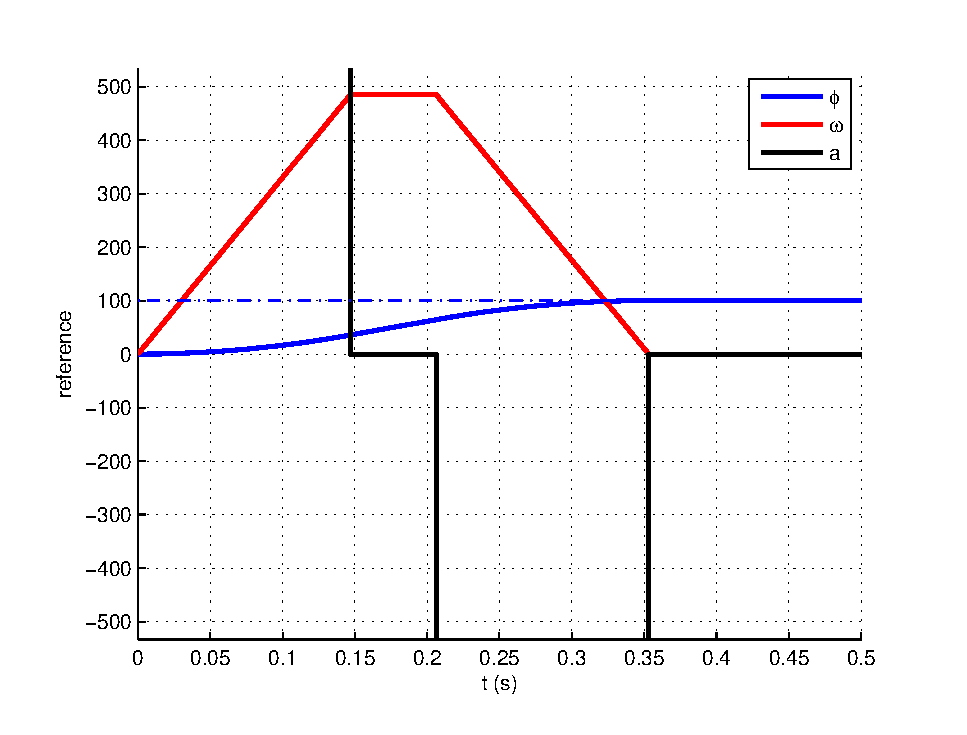
\includegraphics[width = \columnwidth]{fig/trajPlanref100.eps}
  \caption{Reference signal for $Rs = 100$ [rad]}
  \end{subfigure}
  \vspace{\fill}
  \begin{subfigure}[b]{\columnwidth}
  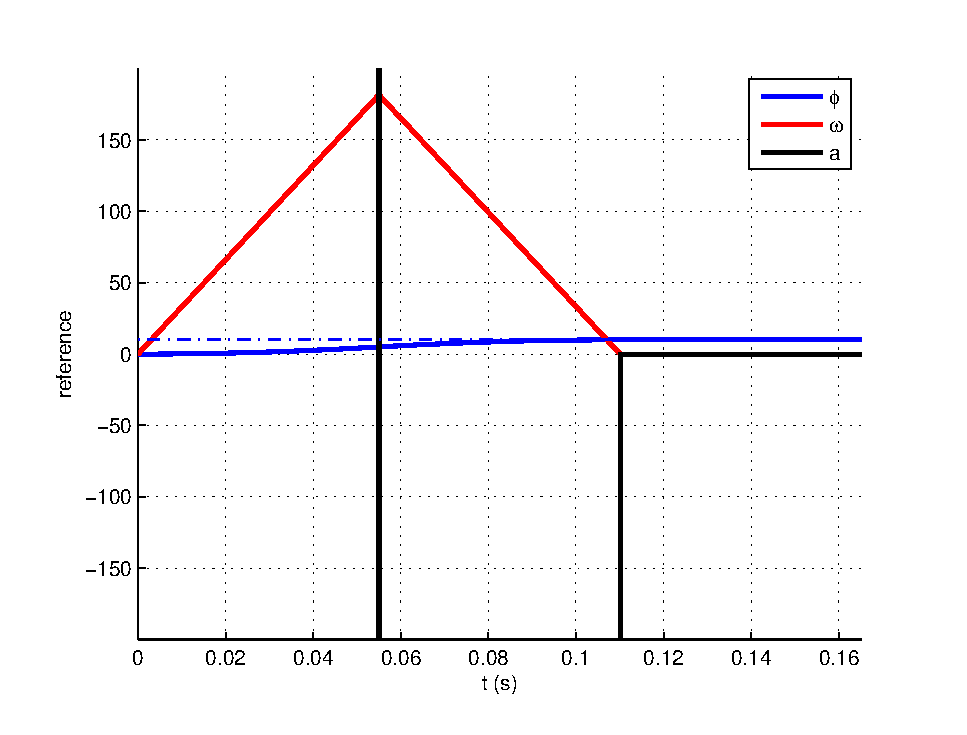
\includegraphics[width = \columnwidth]{fig/trajPlanref10.eps}
  \caption{Reference signal for $Rs = 10$ [rad]}
  \end{subfigure}
\caption{Reference signal}
\label{trajplan}
\end{center}
\end{figure}


Once the reference signal is designed, we simulate the system (simulation and real-case). Figure \ref{resultModelfollowing} shows the results.
 
The Servo control model leads to an excellent control law of the motor for the two set points. Since the trajectory computed by the trajectory planner is completly reachable by the real-motor (no saturation), the planned trajectory and the real one are almost completly merged.

\textbf{Remark:} In order to be sure of our control design, we reduced the value of $a_{max}$ and $v_{max}$ to $75\%$ of the value computed theoretically. Indeed, using the maximum value of those value drive the motor to a dangerous area.

\begin{figure}[ht]
  \centering
  \begin{subfigure}[b]{\linewidth}
   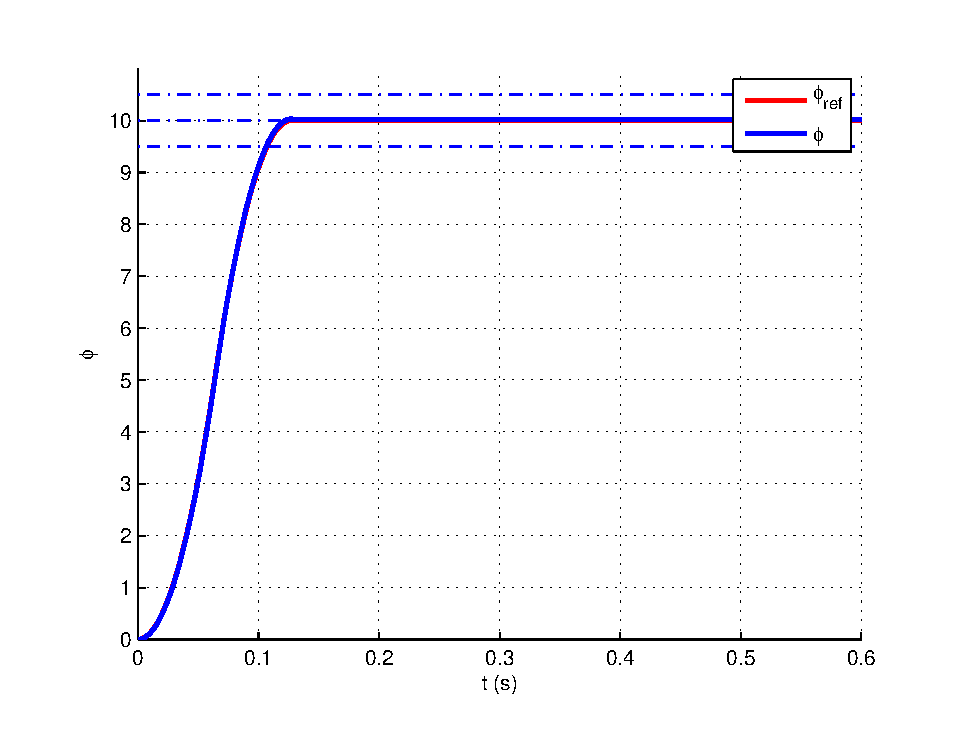
\includegraphics[width=\columnwidth]{fig/resultModelControl10.eps}
   \caption{$Rs = 10$[rad]}
  \end{subfigure}
  \begin{subfigure}[b]{\linewidth}
  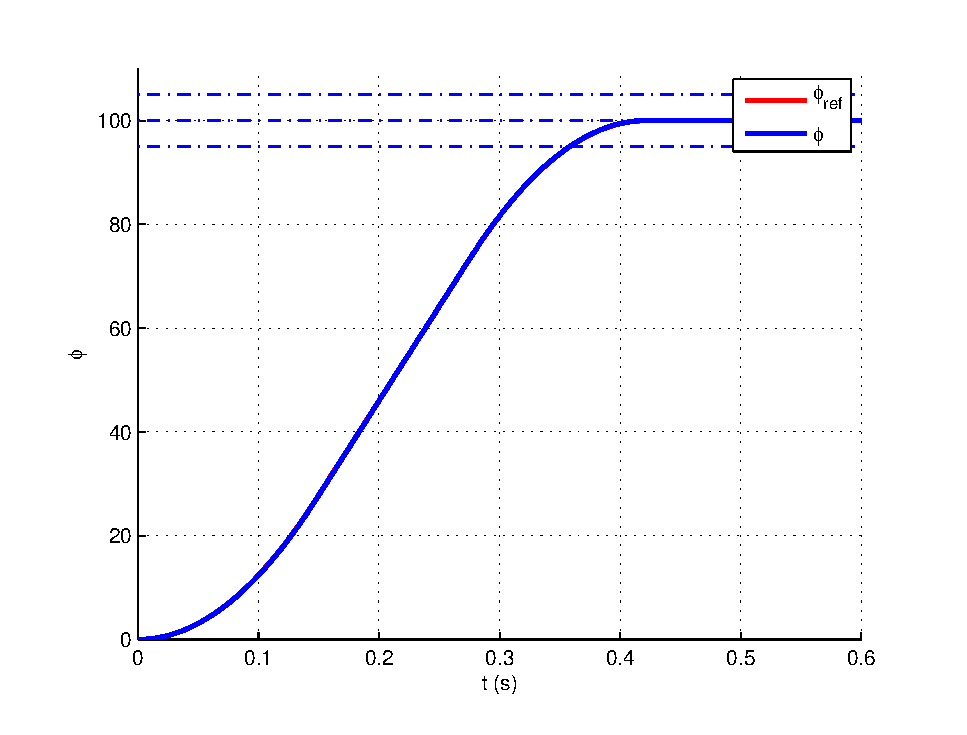
\includegraphics[width=\columnwidth]{fig/resultModelControl100.eps}
   \caption{$Rs = 100$[rad]}
  \end{subfigure}

 \caption{Position controller}
 \label{resultModelfollowing}
\end{figure}



	

\part*{Writing controller code} 
\addcontentsline{toc}{part}{Writing controller code}

%------------------------------------------------
% 		LEVEL 1
%------------------------------------------------
\subsection*{Level 1}
\addcontentsline{toc}{subsection}{Level 1}

The embedded Matlab implementation leads to the exact same result than the implementation using ordinary Simulink blocks. Indeed, since we use a discretize controller, transposing the simulink code to the embedded Matlab implementation produce the a code with the same behavior as the one produced by Simulink.

Figure \ref{embedded} show the superposition of the embedded implementation and the one using Simulink.

See Appendix \ref{appendixCode} for the Matlab code.

\begin{figure}[ht]
  \centering
  \begin{subfigure}[b]{\linewidth}
   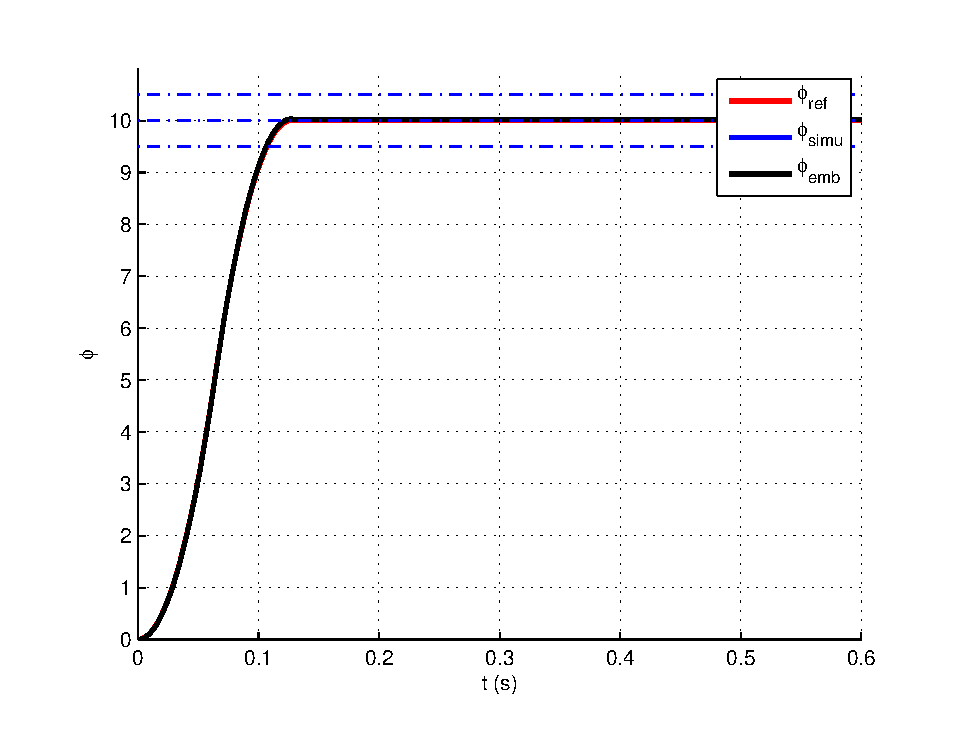
\includegraphics[width=\columnwidth]{fig/embeddedlvl110.eps}
   \caption{$Rs = 10$[rad]}
  \end{subfigure}
  \begin{subfigure}[b]{\linewidth}
  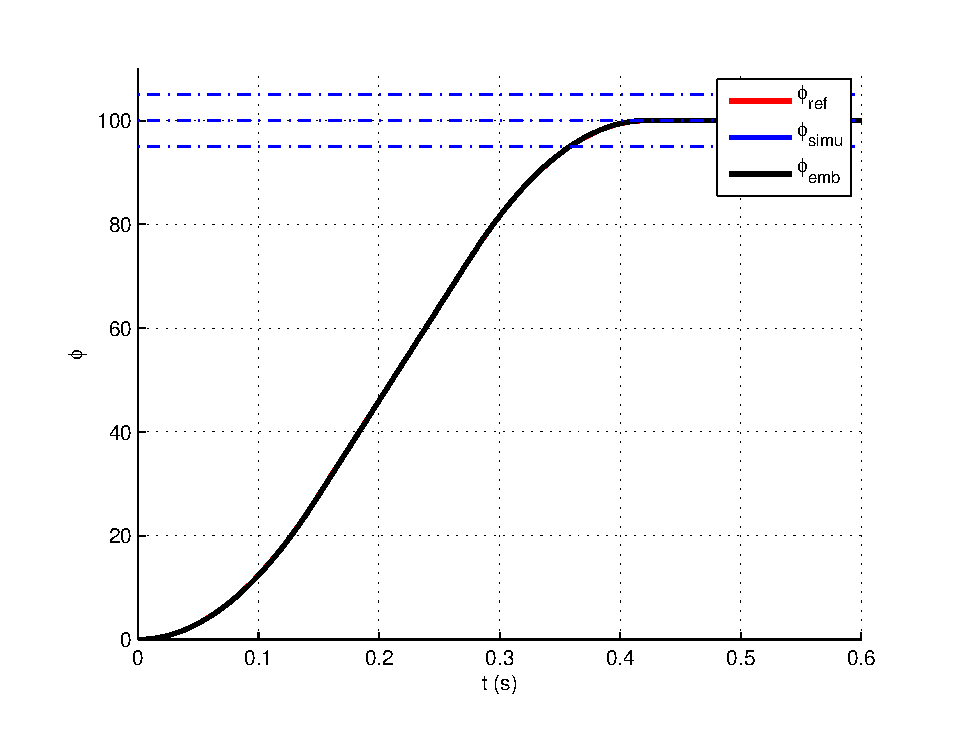
\includegraphics[width=\columnwidth]{fig/embeddedlvl1100.eps}
   \caption{$Rs = 100$[rad]}
  \end{subfigure}

 \caption{Result with a embedded controller}
 \label{embedded}
\end{figure}

%------------------------------------------------
% 		LEVEL 2
%------------------------------------------------
\subsection*{Level 2}
\addcontentsline{toc}{subsection}{Level 2}

Once we had the model following controller with both Simulink and embedded Matlab implementation, we ran it on the real motor. Figure \ref{realresults} shows the two step responses, using the two differents methods. As previously, the two curves are entirely merged.

Moreover, since our controller is designed in such a way that the motor is accelerating at $0.75 a_{max}$ and moving at most at a velocity of $0.75 v_{max}$, the trajectory planner provide safe trajectories. The step response are therefore almost the same as the one simulated.

\begin{figure}[hb]
  \centering
 \begin{subfigure}[b]{\linewidth}
 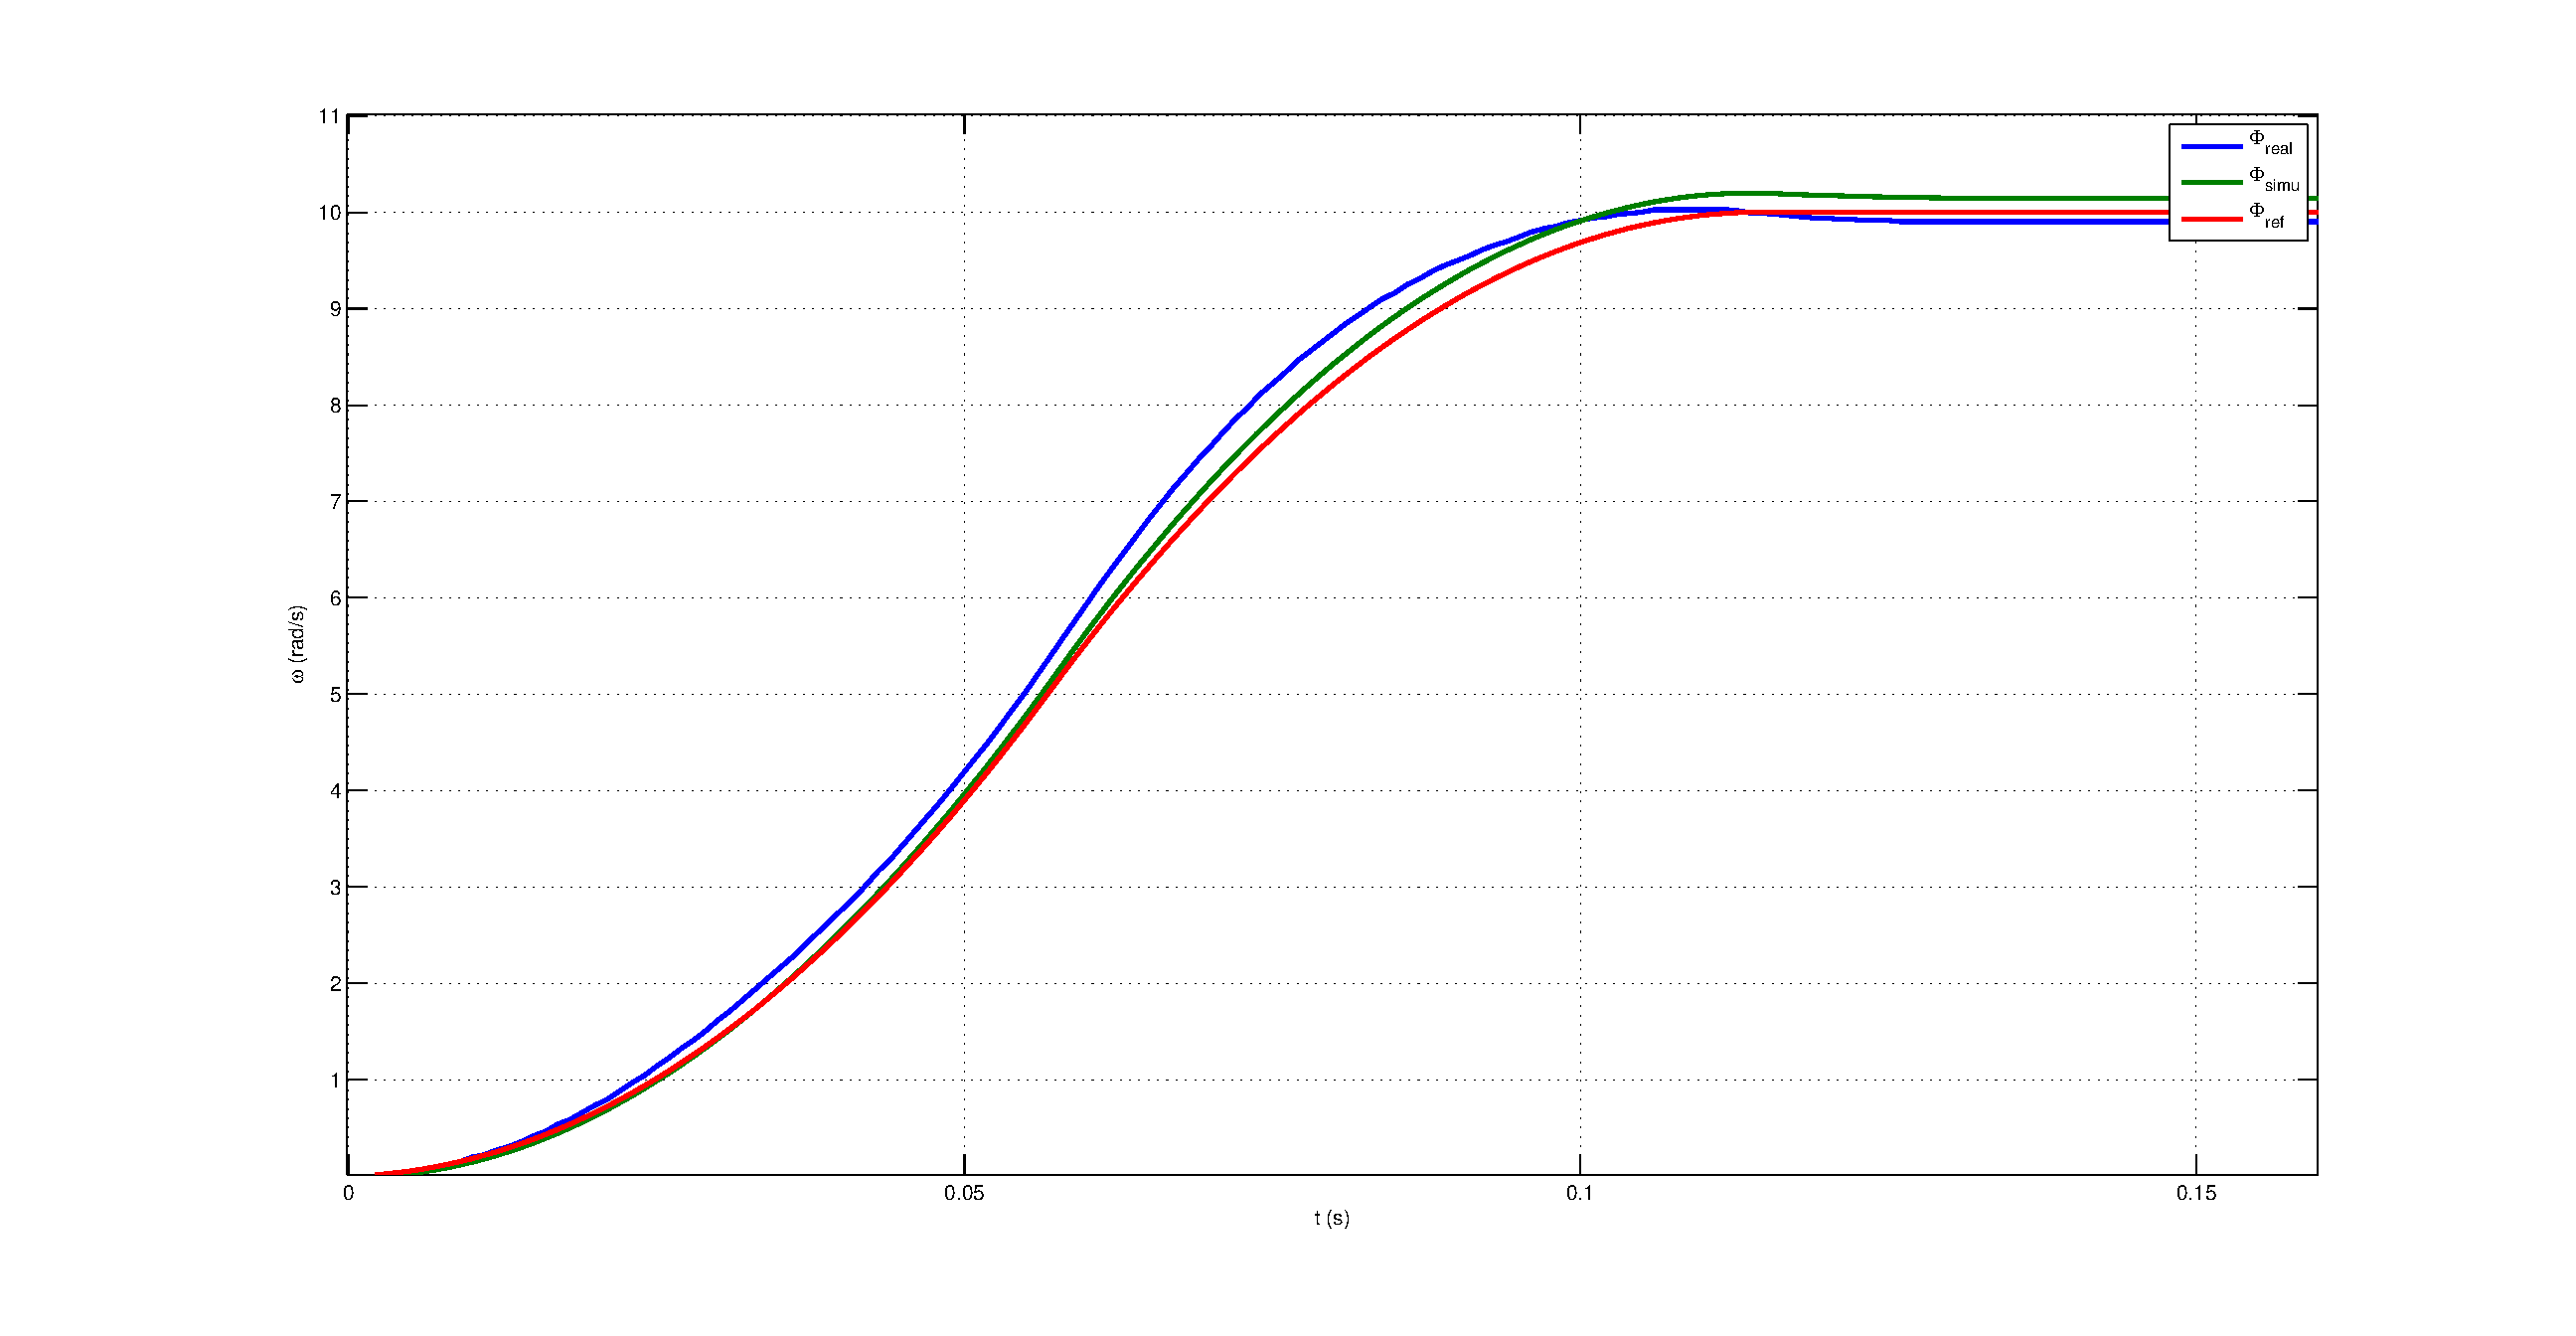
\includegraphics[width=\columnwidth]{fig/10rad.eps}
 \caption{$R_s = 10\text{[rad]}$}
 \end{subfigure}
 \begin{subfigure}[b]{\linewidth}
 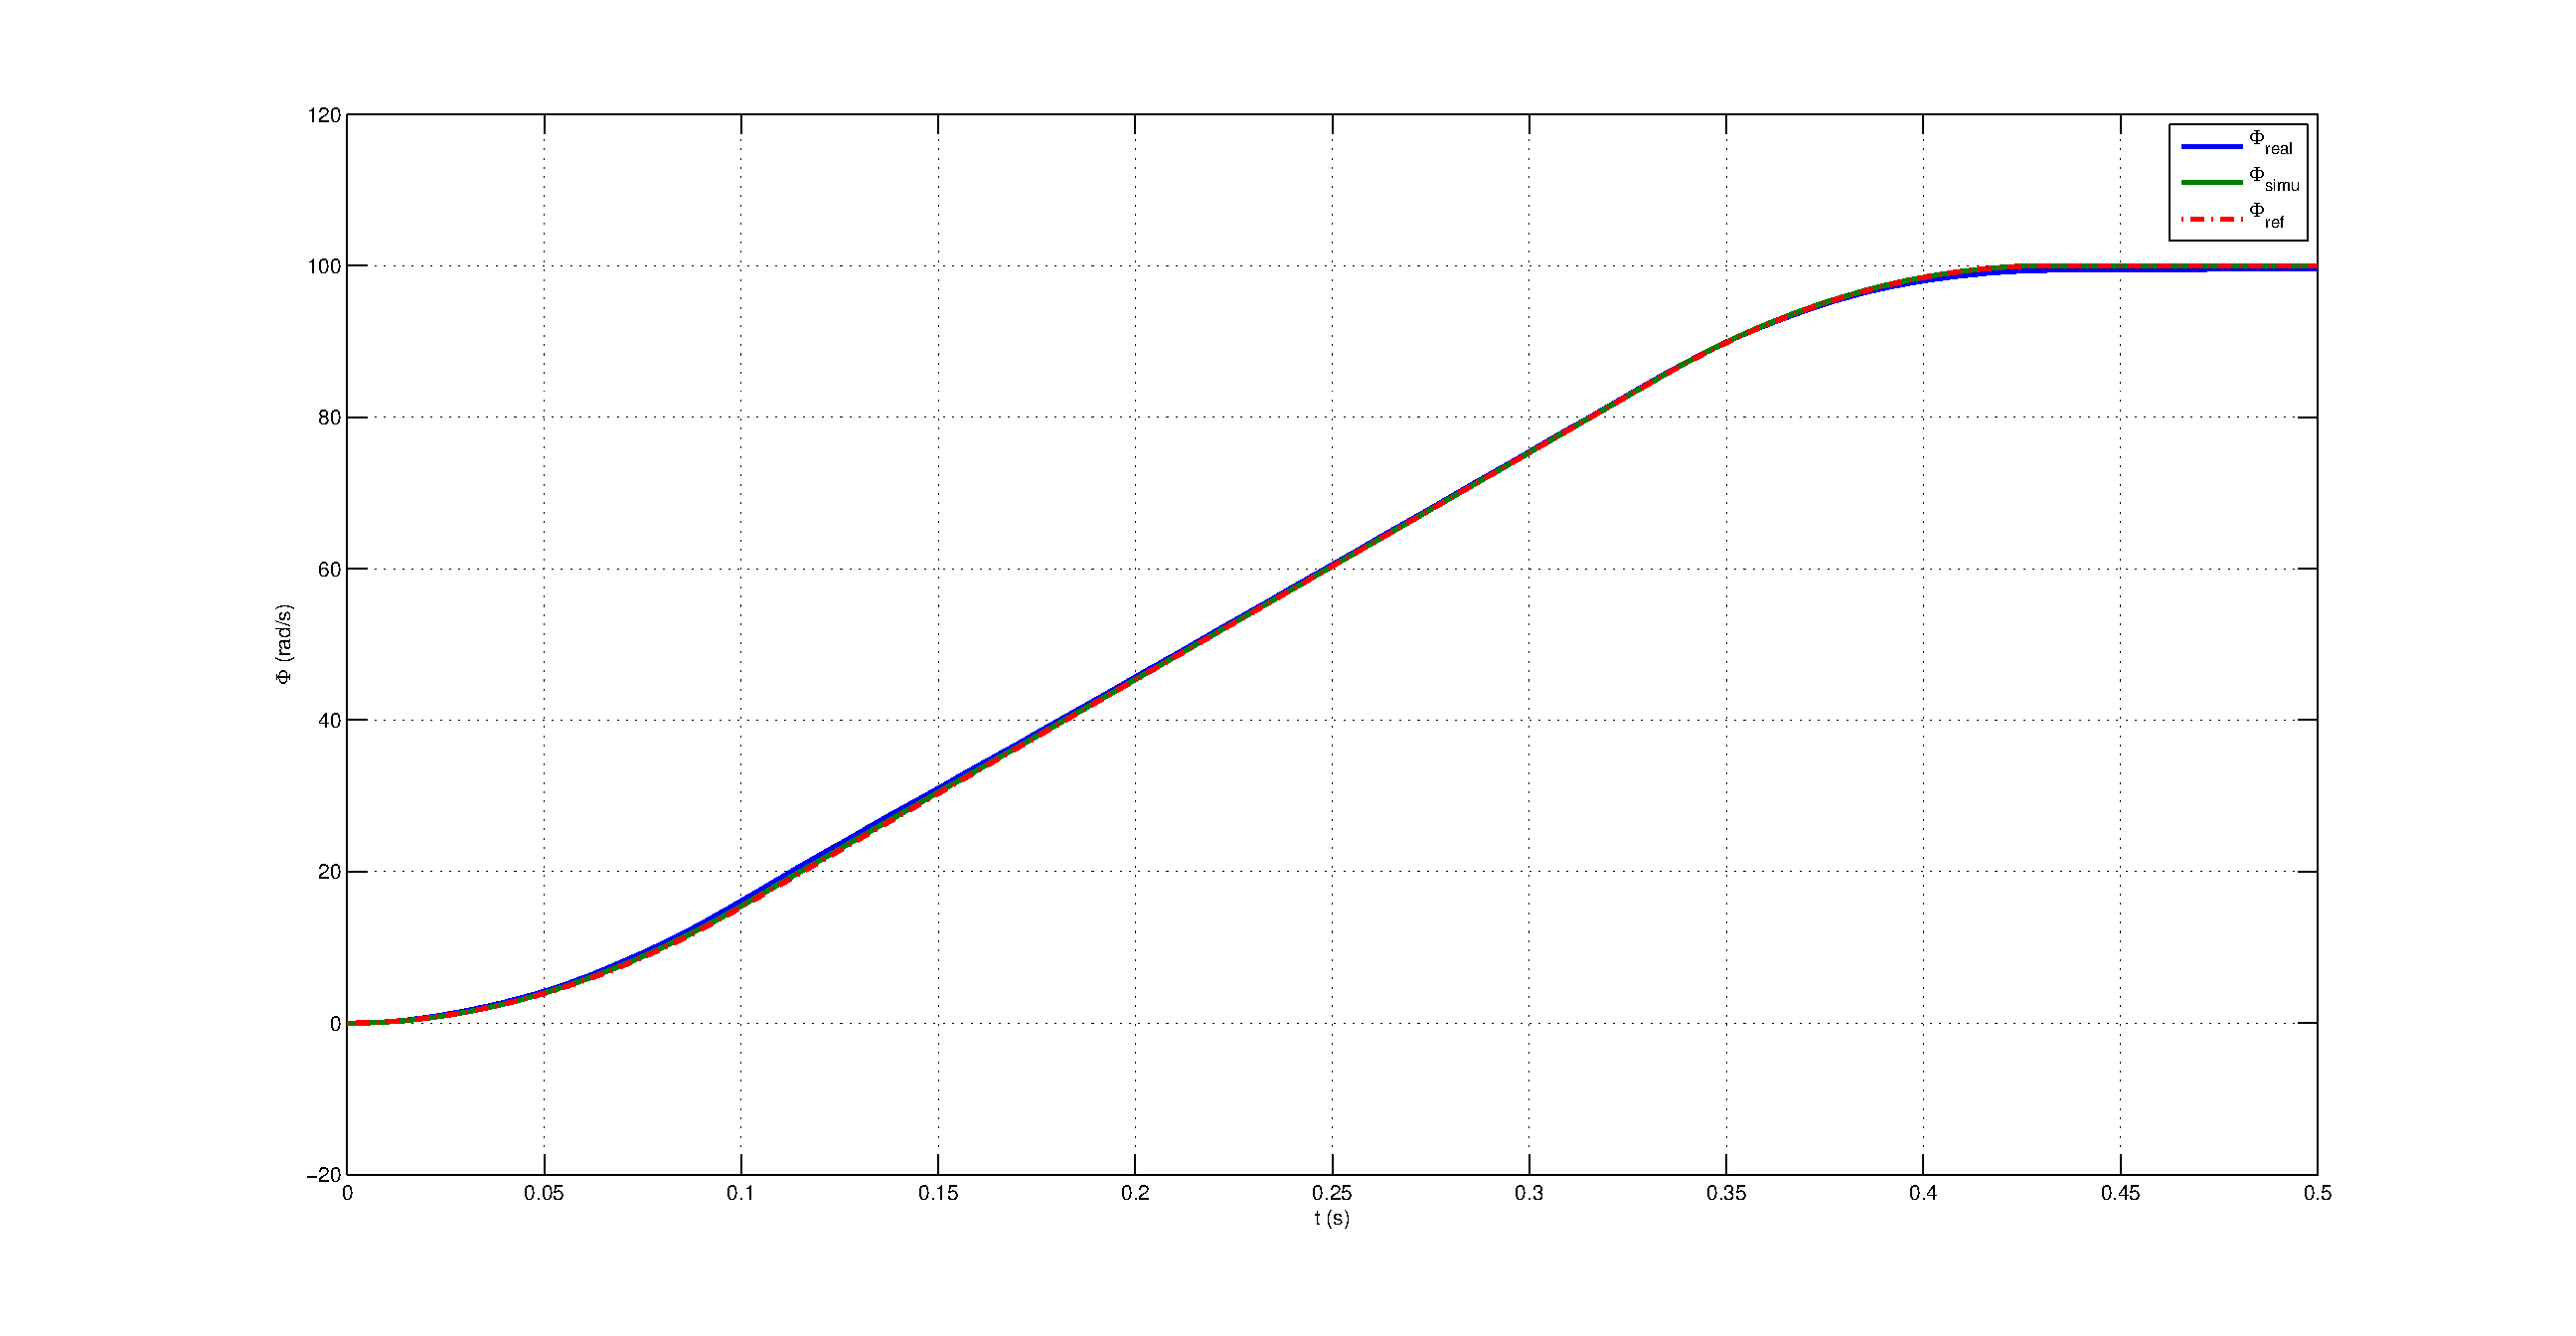
\includegraphics[width=\columnwidth]{fig/100rad.eps}
 \caption{$R_s = 100\text{[rad]}$}
 \end{subfigure}
 \caption{Simulation and real results \\ (blue) -- \\ (green) --}
 \label{realresults}
\end{figure}
	

\clearpage

\part*{Robustness to parameter ncertainty and sensor noise}
\addcontentsline{toc}{part}{Robustness}

This part aims to control a valve for a hydraulic cylinder. Figure \ref{valve} shows the system. 

\begin{figure}[hb]
 \includegraphics[width=\linewidth]{fig/valve.ps}
 \caption{Valve controlled hydraulic cylinder}
 \label{valve}
\end{figure}

%------------------------------------------------
% 		LEVEL 2
%------------------------------------------------
\subsection*{Level 2}
\addcontentsline{toc}{subsection}{Level 2}

We want to design a velocity controller for the valve controlled hydraulic cylinder -- using a continuous controller. 

The system will be simulate using the following reference:
\begin{itemize}
 \item $r(t) = 0.5 \text{ m/s}$
 \item Zero external force
\end{itemize}


%------------------------------------------------
% 		REAL MODEL
%------------------------------------------------
\subsubsection*{Real model}
The system is described by the following equations:

$$
\begin{array}{rcl}
    m \dot{v} & = & p_1 A_1 - p_2 A_2 - d v - f_e \\
    Q_{1v} & = & R_v \sqrt{p_s - p_1} x_v \\
    Q_{2v} & = & R_v \sqrt{p_2 - p_r} x_v \\
    Q_1 & = & Q_{1v} - Q_c \\
    Q_2 & = & - Q_{2v} + Q_c \\
    Q_c & = & A v \\
    C_f \dot{p_1} & = & Q_1 \\
    C_f \dot{p_2} & = & Q_2 \\
\end{array}
$$

With:

$p_i$: internal pression in area $i$

$m$: mass of piston

$A_i$: effective piston area

$f_e$: external force

$d$: friction coefficient

$Q_c$: volume flow due to piston velocity

$Q_{iv}$: flow from/out area $i$

$C_f$: fluid capacitance

$p_s, p_t$: supplied pression, tank pression

$R_v$: flow constant


%------------------------------------------------
% 		LINEAR MODEL
%------------------------------------------------
\subsubsection*{Linear model}
We linearize the model around an operating point:

$$\begin{array}{rcl}
   x_v & = & x_{vQ} + \Delta x_v \\
   p_1 & = & p_{1Q} + \Delta p_1 \\
   p_2 & = & p_{2Q} + \Delta p_2 \\
  \end{array}$$

Let $$x = \left[\begin{array}{ccc}x_1 & x_2 & x_3 \end{array}\right]^T = \left[\begin{array}{ccc} \Delta v & \Delta p_1 & \Delta p_2 \end{array}\right]^T$$ and $$u = \left[\begin{array}{cc}u_1 & u_2 \end{array}\right]^T = \left[\begin{array}{cc} \Delta x_v & f_e \end{array}\right]^T$$

Then:

$$ \begin{array}{rcl} 
    \bm{A} & = & \left(\frac{\partial f_i}{\partial x_j}\right)_{i,j} \\
    \bm{B} & = & \left(\frac{\partial f_i}{\partial u_j}\right)_{i,j}
   \end{array}$$
   
Thus:

$$ \begin{array}{rcl}
    \dot{x} & = &  \bm{A}x + \bm{B}u \\
    y & = & \bm{C}x + \bm{D}u
   \end{array}$$
   
With:

$$\begin{array}{rcl}
   \bm{A} & = & \left(\begin{array}{ccc} 
   -\frac{d}{m} & \frac{A}{m} & -\frac{A}{m} \\ 
   -\frac{A}{C_f} & -\frac{1}{C_f} \frac{R_v x_{vQ}}{2\sqrt{p_s - p_{1Q}}} & 0 \\ 
   \frac{A}{C_f} & 0 & \frac{1}{C_f} \frac{-R_v x_{vQ}}{2 \sqrt{p_{2Q}-p_t}}
   \end{array}\right) \\ \\
   
   \bm{B} & = & \left(\begin{array}{cc}
   0 & \frac{1}{m} \\
   \frac{R_v \sqrt{p_s - p_{1Q}}}{C_f} & 0 \\
   \frac{-R_v \sqrt{p_s - p_{1Q}}}{C_f} & 0 \\
   \end{array}\right) \\ \\
   
   \bm{C} & = & \left(\begin{array}{ccc}
   1 & 0 & 0\\
   \end{array}\right) \\ \\
   
   \bm{D} & = & 0 \\
  \end{array}$$

  
%------------------------------------------------
% 		CONTROL DESIGN
%------------------------------------------------
\subsubsection*{Control design}

% The matrix $\bm{A}$ and $\bm{B}$, using the numerical values, are:
% 
% $$\begin{array}{rcl}
%    \bm{A} & \approx & 1e9 \left(\begin{array}{ccc} 
%    0 & 0 & 0 \\ 
%    -2.86 & 0 & 0 \\ 
%    2.86 & 0 & 0
%    \end{array}\right) \\ \\
%    
%    \bm{B} & \approx & 1e11 \left(\begin{array}{cc}
%    0 & 0 \\
%    5 & 0 \\
%    5 & 0 \\
%    \end{array}\right) \\ \\
%   \end{array}$$
%   
%  \textbf{Remark:} Some values seems to be equal to zero, but are actually really small towards the other ones. Our Matlab implementation does not use zero.
 
 
 
 The close-loop transfert function is equal to:
 
 \begin{multline} 
 H(s) = \frac{B(s)}{A(s)} = \bm{C}(s\bm{I}-\bm{A})^{-1}\bm{B}
%  = \frac{1.807e7}{s^2 + 127s + 1.035e5}
 \end{multline}
  
 The block diagram with the controller is depicted on Figure \ref{bloc}.
 
\begin{figure}[hb]
\begin{tikzpicture}
 \sbEntree{E}
 \sbBloc{TR}{$\frac{T(s)}{R(s)}$}{E}
 \sbRelier[$r$]{E}{TR}
 \sbCompSum*{comp}{TR}{ }{ }{ }{ }
 \sbRelier{TR}{comp}
 \sbBloc{BA}{$H(s) = \frac{B(s)}{A(s)}$}{comp}
 \sbRelier[$u$]{comp}{BA}
 \sbCompSum*[5]{comp2}{BA}{ }{ }{ }{ }
 \sbSortie{S}{comp2}
 \sbRelier[$y$]{comp2}{S}
 \sbDecaleNoeudy[4]{S}{U}
 \sbCompSum*[-4]{comp3}{U}{ }{ }{ }{ }
 \sbBlocr{SR}{$\frac{S(s)}{R(s)}$}{comp3}
 \sbRelieryx{comp2-S}{comp3}
 \sbRelier{comp3}{SR}
 \sbRelierxy{SR}{comp}
 \sbDecaleNoeudy[-2]{comp2}{V}
 \sbRelier[$v$]{V}{comp2}
 \sbDecaleNoeudy[2]{comp3}{N}
 \sbRelier[$n$]{N}{comp3}
 \sbRelier{BA}{comp2}
\end{tikzpicture}
\caption{Block diagram of the system with the controller}
\label{bloc}
\end{figure}

The control law is given by:

$$u(s) = \frac{T(s)}{R(s)} r - \frac{S(s)}{R(s)}y$$

The closed loop response is:

$$y = \frac{B}{AR+BS} r + \frac{AR}{AR+BS}v - \frac{BS}{AR+BS}n$$

Pole placement gives:

\begin{equation} AR + BS = A_m A_0 \label{poleplace} \end{equation}

We start with:

$$
\begin{array}{rcl} A_m(s) & = &  s^2 + 2 \xi_m \omega_m s + \omega_m^2 \\ A_0(s) & = & s + \omega_m' \end{array} 
$$

Therefore since:

$$\begin{array}{rcl} A(s) & =&  s^2 + 2 \xi_0 \omega_0 s + \omega_0^2 \\ B(s) & = & K_0 \end{array}$$

Equation (\ref{poleplace}) leads to:

$$\begin{array}{rcl} R(s) & =&  s+r_c \\ S(s) & = & K_C(s+s_C) \end{array}$$

We then select $T$ such as $T = A_0 t_0$.

Then:

$$\left\{\begin{array}{rcl} 
r_c & = & w_m' + 2(\omega_m \xi_m -\omega_0 \xi_0)  \\
K_C & = & \frac{1}{K_0} \left(\omega_m^2 + 2 \omega_m'^2 \xi_m \omega_m - 2 r_c \xi_0 \omega_0 - \omega_0^2\right) \\
s_C & = & \frac{1}{K_0 K_C}(\omega_m' \omega_m - r_c \omega_0^2) \\
t_0 & = & \frac{\omega_m^2}{K_0}
\end{array}\right.$$


Using the method described in the subject, we obtain the following value (satisfying step response) for $\omega_m$ and $\omega_m'$, leading to the following $A_m$ and $A_0$:

$$\begin{array}{rcl}
   A_m & = & s^2 + 3600s + 4e6 \\
   A_0 & = & s+2e3\\
  \end{array}$$
  
The sensitivity function and the complementary sensitivity function are defined by:

$$\begin{array}{rcl}
   S_e(s) & = & \frac{A(s)R(s)}{A_m(s)A_0(s)} \\
   T_e(s) & = & \frac{B(s)S(s)}{A_m(s)A_0(s)}
  \end{array}$$

Figure \ref{sensitivity} shows the sensitivity function and the complementary sensitivity function bode diagrams.

\begin{figure}[hb]
  \centering
  \begin{subfigure}[b]{\linewidth}
   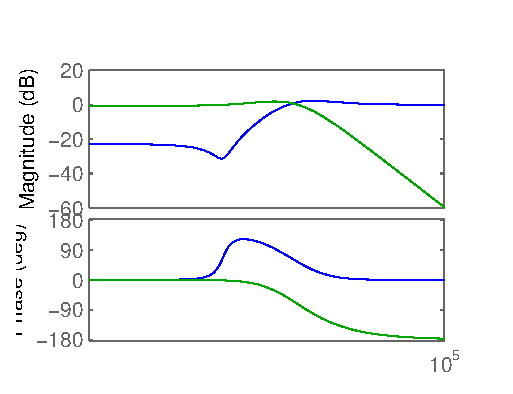
\includegraphics[width=\columnwidth]{fig/bode_SeTe_designAm.eps}
   \caption{$A_0 = s+2e3$}
  \end{subfigure}
  \begin{subfigure}[b]{\linewidth}
  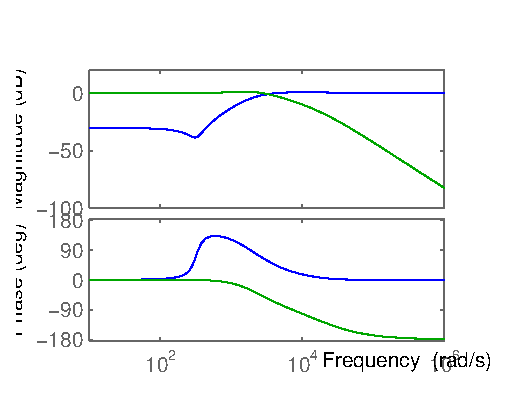
\includegraphics[width=\columnwidth]{fig/bode_SeTe_desginA0.eps}
   \caption{$A_0 = s + 2e4$}
  \end{subfigure}
 \caption{Bode diagram of the Sensitivity and complementary sensitivity functions \\ (green) -- Sensitivity function \\ (blue) -- Complementary sensitivity function }
 \label{sensitivity}
\end{figure}

Figure \ref{stepIdeal} shows the step response of the system without any perturbation. 

\begin{figure}[hb]
  \centering
  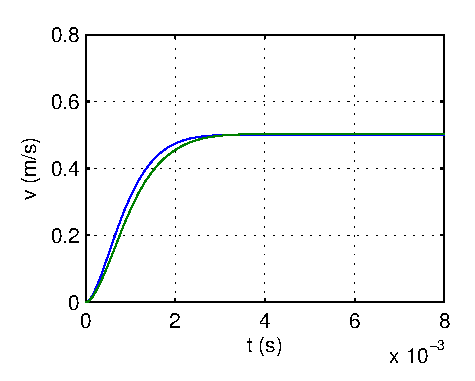
\includegraphics[width=\linewidth]{fig/step_design_Am.eps}
  \caption{Step response of the sytem without any perturbation \\ (green) -- real system \\ (blue) -- linearized system}
  \label{stepIdeal}
\end{figure}

The step responses shows that:
\begin{itemize}
 \item Linearized model and real one are close to each other (the linearization was legitimate a posteriori).
 \item The system react as a second order one (as defined is the design). 
 \item The step responses present no overshoot and are fast.
 \item The non-linearized is almost as fast as the linearized one.
\end{itemize}


\clearpage

%------------------------------------------------
% 		STEP RESPONSE
%------------------------------------------------
\subsubsection*{Step responses with perturbations}

Keeping the same $A_m = s^2 + 3600s + 4e6  $, figure \ref{stepPertu} shows the step responses using a perturbation $f_e = 5000\text{N}$.

\begin{figure}[hb]
  \centering
  \begin{subfigure}[b]{\linewidth}
   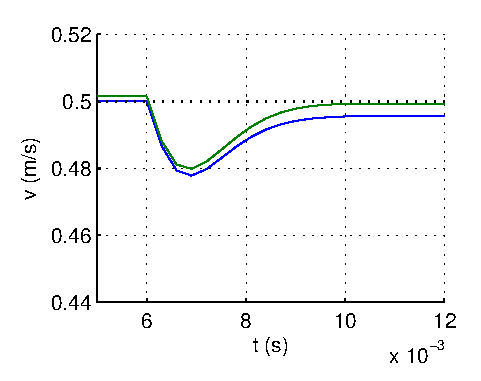
\includegraphics[width=\columnwidth]{fig/step_Fe_AmeqA0.eps}
   \caption{$A_0 = s+2e3$}
  \end{subfigure}
  \begin{subfigure}[b]{\linewidth}
  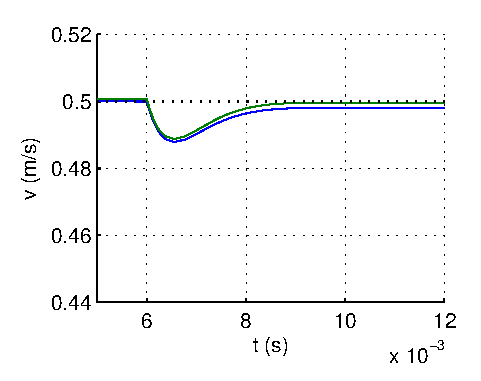
\includegraphics[width=\columnwidth]{fig/step_Fe_w0Eq10wm.eps}
   \caption{$A_0 = s + 2e4$}
  \end{subfigure}
 \caption{Step responses with a perturbation $f_e = 5000 \text{N}$\\ (green) -- real system \\ (blue) -- linearized system}
 \label{stepPertu}
\end{figure}

In the first case ($A_0 = s+2e3$), the steady state error is bigger with the perturbation. This can be explain by the fact that, looking at the bode diagram, the gain is not equal to $- \infty$ with a perturbation.  
But the bigger $\omega_m'$ is, the smaller the gain is. This is why looking at the second step response, we have a smaller steady state error.

Moreover, the system is balancing the perturbation faster with a bigger $\omega_m'$ .

%------------------------------------------------
% 		MASS VARIATION
%------------------------------------------------
\subsubsection*{Mass variation}

We change the mass from $100\text{kg}$ to $200\text{kg}$. Figure \ref{mass} shows the step responses using the two same $A_0$ as in the previous subsubsection.

\begin{figure}[hb]
  \centering
  \begin{subfigure}[b]{\linewidth}
   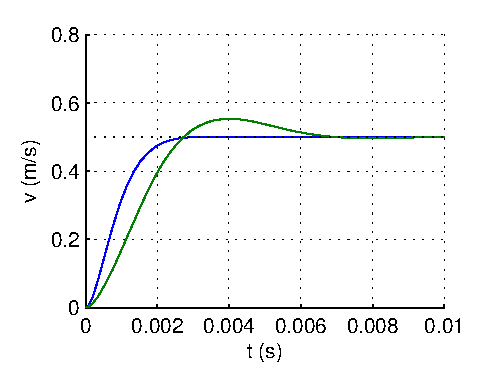
\includegraphics[width=\columnwidth]{fig/step_m_w0eqwm.eps}
   \caption{$A_0 = s+2e3$}
  \end{subfigure}
  \begin{subfigure}[b]{\linewidth}
  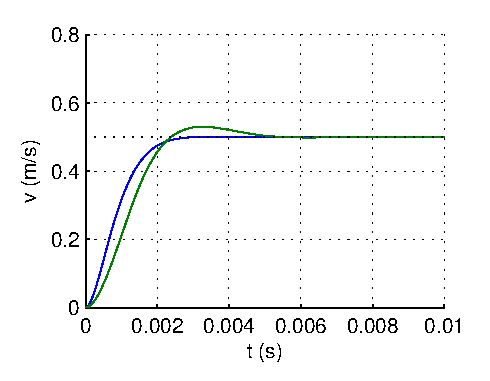
\includegraphics[width=\columnwidth]{fig/step_m_w0eq10wm.eps}
   \caption{$A_0 = s + 2e4$}
  \end{subfigure}
 \caption{Step responses with a $200\text{kg}$ mass \\ (green) -- real system \\ (blue) -- linearized system}
 \label{mass}
\end{figure}

Changing the mass, the linearized system response do not change.

However, the quality of the real system response is damage by this change. Increasing the value of $\omega_m'$ leads to a better step response.

This misestimation of the parameter $m$ can be seens as the addition of noise in the model. As previously, the impact of this noise is reduced by a raise of $\omega_m'$.

%------------------------------------------------
% 		NOISE EFFECT
%------------------------------------------------
\subsubsection*{Noise effect}

In order to analyse the impact of the noise in our system, we added some in the feedback loop. Figure \ref{noise} shows the step responses with two different $A_0$.

\begin{figure}[hb]
  \centering
  \begin{subfigure}[b]{\linewidth}
   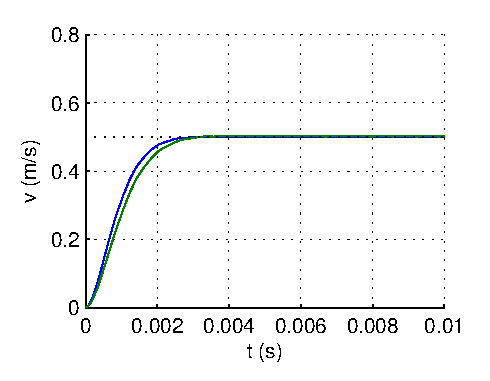
\includegraphics[width=\columnwidth]{fig/step_wm_noise.eps}
   \caption{$A_0 = s+2e3$}
  \end{subfigure}
  \begin{subfigure}[b]{\linewidth}
  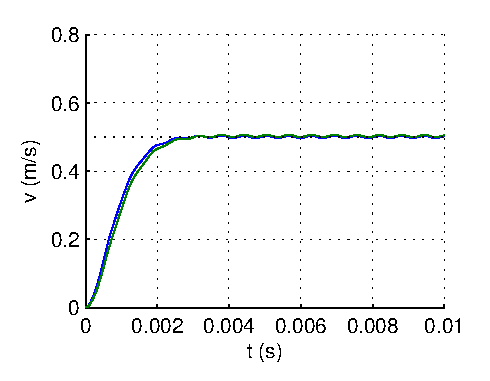
\includegraphics[width=\columnwidth]{fig/step_10wm_noise.eps}
   \caption{$A_0 = s + 2e4$}
  \end{subfigure}
 \caption{Step responses with noise \\ (green) -- real system \\ (blue) -- linearized system}
 \label{noise}
\end{figure}


The system response is worse in the second case ($\omega_m' = 2e4$). Indeed, the bode diagram shows that the cutoff frequency in this case is bigger than in the other case. The bigger $\omega_m'$, the more the noise impacts the system response.






\clearpage

\end{document}
